\chapter{Methods}

 1. Data
  	
  	- Bedmap3 along-track picks rather than a gridded product~\cite{Pritchard_2025}
	
	- \texttt{processing\_flag}: migration status, uniform per CSV
  	
  	- Seven regions with boundaries~\cite{Ockenden_2025_data}

	- REMA and MEaSUREs

2. Processing and Analysis

	- ANALYSIS UNIT: 50 km sliding window at 50\% overlap

	- Landscape splitting via gradient segmentation and the limitation of excluded
    transition windows. Relief is \texttt{elevation\_max - elevation\_min} with no detrend, so
    on a straddling window it returns the elevation offset between two terrains
    rather than the elevation range within either one.

	- Survey grading: \texttt{coverage\_tags.py}, A/B/C tiers on interpolation distance,
   azimuth concentration and homogeneous window count,

   - Spectral method

\begin{figure}[H]
    \includegraphics[scale=0.038]{figures/Fig2.png}
    \caption{} 
    \label{fig:pipeline_workflow}
\end{figure}

3. The vector elements:
\begin{table}[htbp]
\centering
\caption{Classification axes and descriptors of the landscape classification vector}
\label{tab:axes_descriptors}
\begin{tabularx}{\textwidth}{l p{3.5cm} X}
\toprule
\textbf{Category} & \textbf{Variable} & \textbf{Description / Threshold} \\
\midrule
\textbf{Classifying axes} 
  & \texttt{$\beta$} & The spectral slope is a first-order summary of basal character. High $\beta$ indicates smooth, soft beds (sedimentary basins, active ice streams), while low $\beta$ indicates hard, jagged crystalline shields (e.g., Jordan et al. (2017)~\cite{Jordan_2017}; Bingham et al (2009)~\cite{Bingham_2009}). \\
  \addlinespace[0.5em]
  & \texttt{relief\_m} & \\
  \addlinespace[0.5em]
  & \texttt{bed\_elev\_mean} & \\
  \addlinespace[0.5em]
  & \texttt{measures\_speed\_mean} & \\
\midrule
\textbf{Descriptors} 
  & \texttt{A\_1km} & The roughness amplitude is necessary to separate features like flat crystalline plains from mountainous rift flanks (e.g., Cooper et al (2019)~\cite{Cooper_2019}). \\
  \addlinespace[0.5em]
  & \texttt{rms\_roughness} & \\
  \addlinespace[0.5em]
  & \texttt{xi\_band} & \\
  \addlinespace[0.5em]
  & \texttt{eta\_wavelength\_m} & \\
  \addlinespace[0.5em]
  & \texttt{hill\_count} & \\
  \addlinespace[0.5em]
  & \texttt{skewness} & \\
  \addlinespace[0.5em]
  & \texttt{kurtosis} & \\
\bottomrule
\end{tabularx}
\end{table}



%  \begin{itemize}
 
%  \item Classifying axes and their thresholds
%     \begin{enumerate}

%     \item{\texttt{$\beta$}}: The spectral slope is a first-order summary of basal character. High $\beta$ indicates smooth, soft beds (sedimentary basins, active ice streams), while low $\beta$ indicates hard, jagged crystalline shields (e.g., Jordan et al. (2017)~\cite{Jordan_2017}; Bingham et al (2009)~\cite{Bingham_2009}). 

%     \item{\texttt{relief\_m}}:

%     \item{\texttt{bed\_elev\_mean}}:
    
%     \item{\texttt{measures\_speed\_mean}}:

%     \end{enumerate}

% \item Descriptors

%     \begin{enumerate}

%     \item{\texttt{A\_1km}}: The roughness amplitude is necessary to separate features like flat crystalline plains from mountainous rift flanks (e.g., Cooper et al (2019)~\cite{Cooper_2019}).

%     \item{\texttt{rms\_roughness}}:

%     \item{\texttt{xi\_band}}:

%     \item{\texttt{eta\_wavelength\_m}}:

%     \item{\texttt{hill\_count}}:

%     \item{\texttt{skewness}}:

%     \item{\texttt{kurtosis}}:

%     \end{enumerate}
%     \end{itemize}

	- The descriptors are continuous because I found no defensible literature threshold.

	- Dependence structure of vector elements:
% \begin{figure}[H]
%     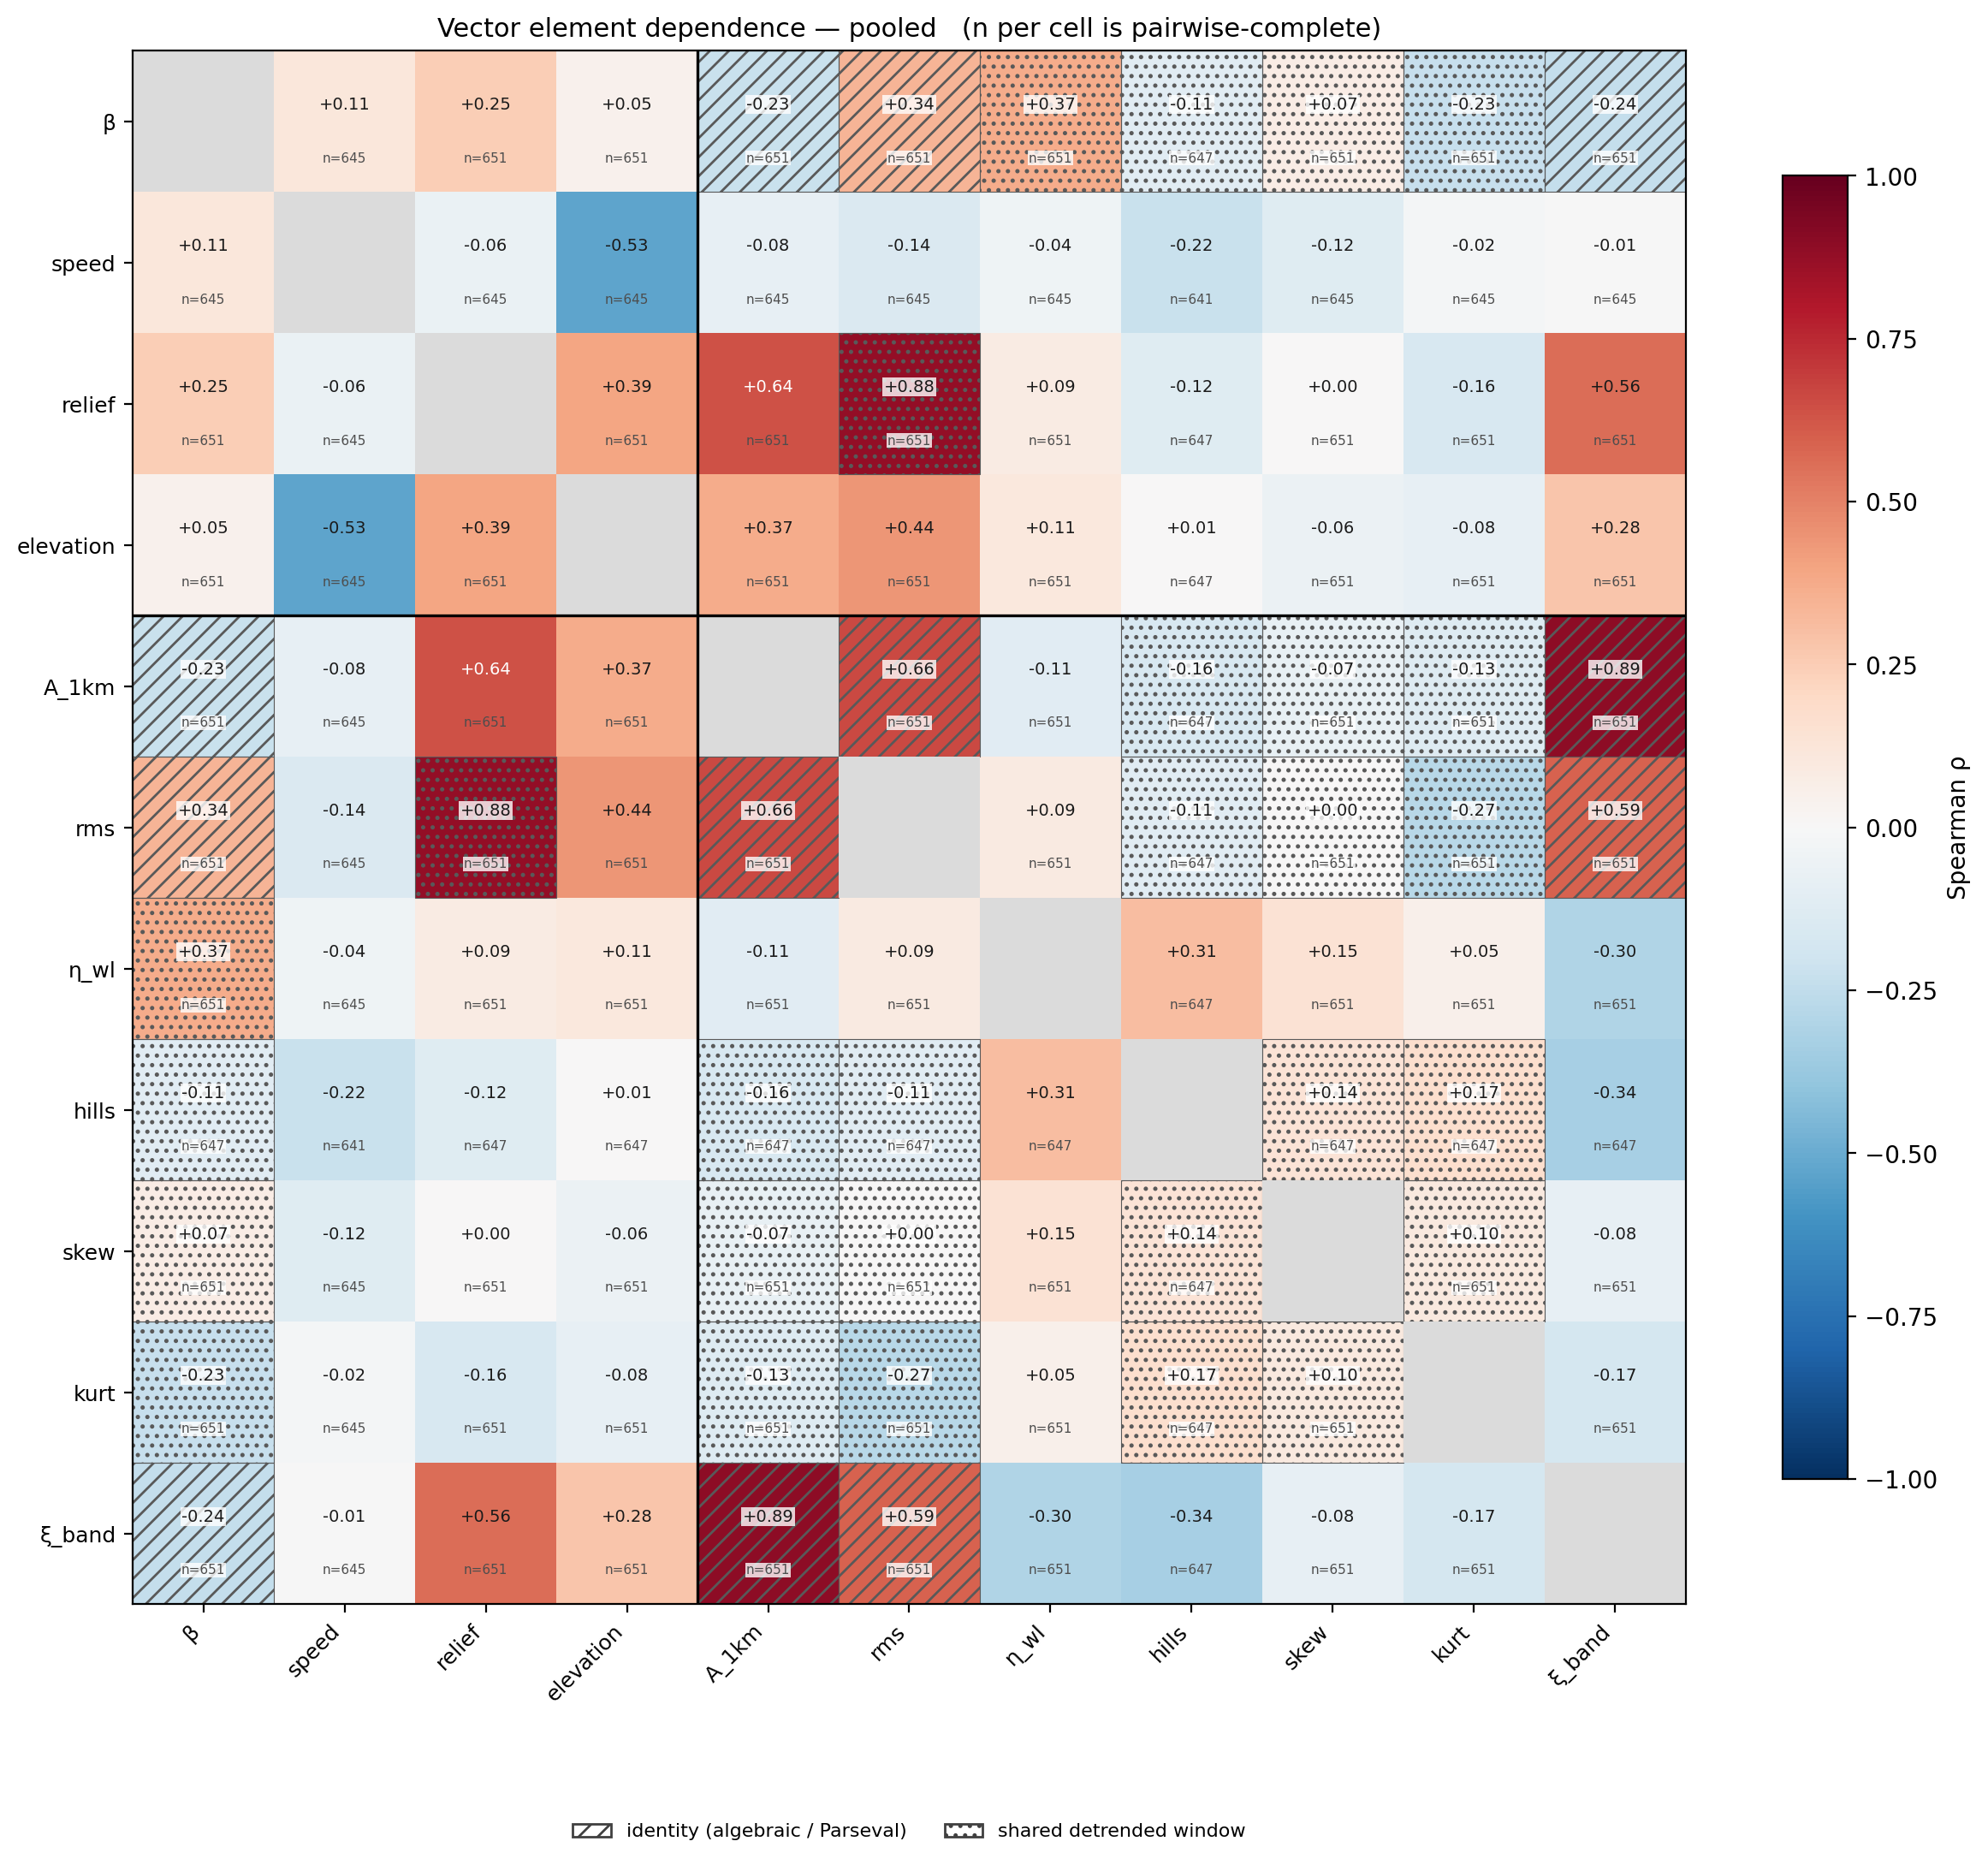
\includegraphics[scale=0.58]{figures/vector_independence_matrix.png}
%     \caption{} 
%     \label{fig:independence_matrix}
% \end{figure}